\documentclass[conference,compsoc,final,a4paper]{IEEEtran}
\usepackage[utf8]{inputenx}
\usepackage{float} % for Table float parameter H

%% Bitte legen Sie hier den Titel und den Autor der Arbeit fest
\newcommand{\autoren}[0]{Karhan, Marvin}
\newcommand{\dokumententitel}[0]{Welchen Einfluss haben Dark Patterns auf Nutzer?}

% Hie muss normalerweise nichts angepasst werden
\usepackage[pdftex]{graphicx}
\graphicspath{{img/}}
\DeclareGraphicsExtensions{.pdf,.jpeg,.jpg,.png}
\usepackage[cmex10]{amsmath}
\usepackage{algorithmic}
\usepackage{array}
\usepackage{dblfloatfix}
\usepackage{url}
\usepackage[autostyle=true,german=quotes]{csquotes}
\usepackage[backend=biber,
            sorting=none,   % Keine Sortierung
            doi=true,       % DOI anzeigen
            isbn=false,     % ISBN nicht anzeigen
            url=true,       % URLs anzeigen
            maxnames=6,     % Ab 6 Autoren et al. verwenden
            minnames=1,     % und nur den ersten Autor angeben
            style=ieee,]{biblatex}
\usepackage{booktabs}
\usepackage{xcolor}
\usepackage{listings}             % Source Code listings
\usepackage[printonlyused]{acronym}
\usepackage{fancyvrb}
\usepackage{tocloft} % Schönere Inhaltsverzeichnisse

% Farben definieren
\definecolor{linkblue}{RGB}{0, 0, 100}
\definecolor{linkblack}{RGB}{0, 0, 0}
\definecolor{darkgreen}{RGB}{14, 144, 102}
\definecolor{darkblue}{RGB}{0,0,168}
\definecolor{darkred}{RGB}{128,0,0}
\definecolor{comment}{RGB}{63, 127, 95}
\definecolor{javadoccomment}{RGB}{63, 95, 191}
\definecolor{keyword}{RGB}{108, 0, 67}
\definecolor{type}{RGB}{0, 0, 0}
\definecolor{method}{RGB}{0, 0, 0}
\definecolor{variable}{RGB}{0, 0, 0}
\definecolor{literal}{RGB}{31,0, 255}
\definecolor{operator}{RGB}{0, 0, 0}

\usepackage[ngerman]{betababel}

\DefineBibliographyStrings{ngerman}{
    andothers = {{et al\adddot}},  % Immer et al. sagen, auch bei Deutsch als Sprache
}
\usepackage[
      unicode=true,
      hypertexnames=false,
      colorlinks=true,
      colorlinks=false,
      linkcolor=darkblue,
      citecolor=darkblue,
      urlcolor=darkblue,
      pdftex
   ]{hyperref}
%	 \PrerenderUnicode{ü}


% Einstellungen für Quelltexte
\lstset{
    xleftmargin=0.1cm,
    basicstyle=\scriptsize\ttfamily,
    keywordstyle=\color{keyword},
    identifierstyle=\color{variable},
    commentstyle=\color{comment},
    stringstyle=\color{literal},
    tabsize=2,
    lineskip={2pt},
    columns=flexible,
    inputencoding=utf8,
    captionpos=b,
    breakautoindent=true,
    breakindent=2em,
    breaklines=true,
    prebreak=,
    postbreak=,
    numbers=none,
    numberstyle=\tiny,
    showspaces=false,      % Keine Leerzeichensymbole
    showtabs=false,        % Keine Tabsymbole
    showstringspaces=false,% Leerzeichen in Strings
    morecomment=[s][\color{javadoccomment}]{/**}{*/},
    literate={Ö}{{\"O}}1 {Ä}{{\"A}}1 {Ü}{{\"U}}1 {ß}{{\ss}}2 {ü}{{\"u}}1 {ä}{{\"a}}1 {ö}{{\"o}}1
}

\hypersetup{
    pdftitle={\dokumententitel},
    pdfauthor={\autoren},
    pdfdisplaydoctitle=true,
    hidelinks
}

% Makros für typographisch korrekte Abkürzungen
\newcommand{\zb}[0]{z.\,B.\ }
\newcommand{\dahe}[0]{d.\,h.\ }
\newcommand{\ua}[0]{u.\,a.\ }

% Wo liegt Sourcecode?
\newcommand{\srcloc}{src/}

% Literatur einbinden
\addbibresource{literatur.bib} % Weitere Einstellungen aus einer anderen Datei lesen

\begin{document}

% Titel des Dokuments
\title{\dokumententitel}

% Namen der Autoren
\author{
  \IEEEauthorblockN{\autoren}
  \IEEEauthorblockA{
    Hochschule Mannheim\\
    Fakultät für Informatik\\
    Paul-Wittsack-Str. 10,
    68163 Mannheim
  }
}

% Titel erzeugen
\maketitle
\thispagestyle{plain}
\pagestyle{plain}

% Eigentliches Dokument beginnt hier
% ----------------------------------------------------------------------------------------------------------

% Kurze Zusammenfassung des Dokuments
\begin{abstract}
Abstract
\end{abstract}

% Inhaltsverzeichnis erzeugen
{\small\tableofcontents}

% Abschnitte mit \section, Unterabschnitte mit \subsection und
% Unterunterabschnitte mit \subsubsection
\section{Einleitung}
"“Dark pattern” means a user interface designed or manipulated with the substantial effect of subverting or impairing user autonomy, decisionmaking, or choice"

\section{Zusätzliche Angaben}
\subsection{Zentrale Begriffe}
\begin{itemize}
\item Dark Pattern
\item Anti-Pattern
\item evil design
\item black hat UX
\item dark ux
\item Marktpsychologie
\item CCPA (California Consumer Privacy Act)
\item GDPR (General Data Protection Regulation)
\item Persuasive design
\item Deceptive design
\item Human-centered computing
\item Human computer interaction (HCI)
\end{itemize}

\subsection{Zeitplan}
Generell ist vor jeder textuellen Abgabe entsprechend dem Umfang der Abgabe eine Rechtschreibprüfung eines Dritten angesetzt.
\begin{table}[H]
\begin{tabular*}{\linewidth}{ @{\extracolsep{\fill}}l  l}
    \toprule
\textbf{Zeitraum}                   & \textbf{Geplante Tätigkeit}       \\
    \midrule
16.04 - 23.04                       & Weitere Literaturrecherche        \\
24.04 - 30.04                       & Kapitel 3.0 (Kapiteleinleitung), 3.1                          \\
01.05 - 14.05                       & Kapitel 3.2 - 3.4                          \\
\textbf{14.05}                      & \textbf{Abgabe des Probekapitels} \\
15.05 - 28.05                       & Kapitel 4                           \\
29.05 - 11.06                       & Kapitel 5                          \\
12.06 - 25.06                       & Kapitel Abstract und Einleitung                          \\
\textbf{25.06}                      & \textbf{Abgabe zum Peer-Review}   \\
\textbf{07.07}                      & \textbf{Peer-Review (8:00 - 11:15 Uhr)} \\
\textbf{08.07}                      & \textbf{Abgabe der Peer-Review-Bögen}   \\
09.07 - 16.07                       & Einarbeitung der Kritik und letzte Verbesserungen                           \\
\textbf{16.07}                      & \textbf{Abgabe des fertigen Papers}      \\
    \bottomrule
\end{tabular*}
\end{table}

\subsection{Kontextabgrenzung}
Dieses Paper vermittelt einen Einblick in die Konzepte, die das Fundament für die Definition des Dark Pattern Begriffes liefern. Wie sich Dark Patterns in Applikationen manifestieren und wie Verbraucher vor Missbrauch durch Dark Patterns geschützt werden, bzw. wie können sich Nutzer davor schützen. Außerdem wird im Ausblick darauf eingegangen wie Regularien oder Nutzerverhalten den Einsatz von Dark Patterns in Zukunft beeinflussen kann.

\section{Dark Patterns Grundlagen}
% // David Brignull als Erfinder des Begriffs 2010\\
% // wer setzt das warum ein\\
Designer machen nur, was von ihnen gefordert wird. Wenn sie es nicht tun, werden es andere tun \autocite{Nerdwriter1_YT_2018}. Nutzer lesen nicht jedes Wort auf einer Webseite, sie überfliegen und machen Annahmen \autocite{Brignull}. Firmen können das ausnutzen, indem sie die Seite anders aussehen lassen, als was sie tatsächlich aussagt \autocite{Brignull}.

Firmen setzen Dark Patterns unter anderem für Growth Hacking ein. In einem digitalen Umfeld ist dafür oft A/B-Testing das Mittel der Wahl, da so Annahmen mit Nutzerdaten untermauert werden können. Das führt dazu, dass Designer unbewusst und ohne eine böse Absicht Dark Patterns in die Webseite einfügen. \autocite{Narayanan2020}

Dieses Kapitel ordnet Dark Patterns ein, beschreibt wie die Grundfesten der menschlichen Psyche ausgenutzt werden können, was \textit{Nudging} ist und anhand eines Beispiels wie \textit{Nudges} eingesetzt werden können.
\subsection{Anti-Pattern}
% // Anti-Pattern als Überbegriff von Dark Pattern und Einleitung in das Thema\\
Ein Pattern ist der Bauplan einer Lösung zu einem wiederkehrenden Problem. Sie existieren in vielen Anwendungsbereichen \autocite[S. 1]{MacDonald2019}.

Anti-Pattern sind ein Sammelbegriff für Pattern, welche wiederkehrende Lösungen liefern, aber dabei mehr Probleme erzeugen als lösen \autocite[S. 193-195]{MacDonald2019}. Wie sich aus dem Namen bereits erschließen lässt, sind Dark Patterns eine spezifische Pattern Art. Dark Patterns erzeugen in erster Linie Probleme für den Nutzer. Die Probleme, die sie lösen wollen, liegen auf der Seite derjenigen, die sie einsetzen. Weil hierbei der Nutzer ausgenutzt und Profit über Nutzerfreundlichkeit gestellt wird \autocite{Chivukula_2019}, zählen Dark Patterns zu der Familie der Anti-Pattern.
\subsection{Psychologie}
\label{chap:Psychologie}
% // Warum spielt Psychologie eine rolle bei Dark Patterns?
% \\// Wie werden Nutzer von Dark Pattern beeinflusst?
% \\// Diskussion verschiedener erhobenen Statistiken zu Nutzerverhalten:\\
Dark Patterns nutzen menschliches Verhalten aus, um Nutzer zu bewegen, etwas ungewollt oder unbewusst zu tun \autocite{Brignull}. Dafür nutzen sie oft kognitive Verzerrung. Kognitive Verzerrung beschreibt, wie mithilfe von Effekten und Techniken die Denkweise unseres Gehirns ausgenutzt werden kann \autocite{Mathur2019}.

Eine weit verbreitete psychologische Technik im Einzelhandel ist die psychologische Preisgestaltung. Das heißt der Preis eines Produkts wird minimal, unter einer runden Zahl angesetzt. Diese Technik ist schon seit mehreren Jahrzehnten im Einsatz und laut \citeauthor{Bizer_2005} (\citedate{Bizer_2005}) \autocite{Bizer_2005} ein effektives Mittel zur Verkaufssteigerung. Im Gegensatz dazu steht \citeauthor{Wieseke_2015} \autocite{Wieseke_2015} Studie aus dem Jahr \citedate{Wieseke_2015}, die sagt: Runde Preise sorgen für die höchstmögliche Verkaufswahrscheinlichkeit, da diese bequemer für den Käufer sind. Ein vergleichbarer Effekt kann bei Dark Patterns auftreten. Im ersten Schritt sorgt der Einsatz von Dark Patterns für eine höhere Nutzerbindung, jedoch im zweiten Schritt zu einer gegenläufigen Wirkung \autocite{M.Bhoot2020}.

Schon in der Zeit vor der Digitalen Revolution wurden die Effekte kognitiver Verzerrung untersucht. Die Ergebnisse dieser Untersuchungen geben Aufschluss über die Manifestierung von Dark Patterns in der menschlichen Psyche.

\citeauthor{Tversky453} zeigen in ihrer Untersuchung, wie die Darstellung eines Problems ihr Ergebnis beeinflusst. Sie zeigen, dass Probanden auf zwei Probleme mit dem faktisch gleichen Ergebnis, in Problem eins eine andere Auswahl als in Problem zwei treffen, obwohl sich nur die Darstellung des Problems geändert hat \autocite{Tversky453}. Diese psychologische Betrachtung lässt sich leicht auf Dark Patterns ausweiten, da Designer in einem Webumfeld weitreichende Möglichkeiten haben, um die Information, die übermittelt werden soll, so zu vermitteln, dass der Nutzer nur durch ihre Darstellung zu einem anderen Ergebnis gedrängt wird.
\subsection{Nudging}
% // Vorhersehbares Beeinflussen von Nutzern um ein gewünschtes Ziel zu erreichen\\
Richard H. Thaler ist Nobelpreisträger für Wirtschaftswissenschaften. Er ist zusammen mit Cass R. Sunstein der Autor des Buchs \citetitle{Thaler2008}, der den Begriff \textit{Nudge} geprägt hat.

Er bezeichnet Personen, die Macht über den Kontext haben, indem sie andere Entscheidungen treffen als \textit{choice architects} \autocite[S. 3]{Thaler2008}. Im Fall von Dark Patterns sind meistens Designer diejenigen, die Thaler und Sunstein als \textit{choice architects} bezeichnen. Ihre Werkzeuge sind die in \autoref{chap:Psychologie} angeschnittenen psychologischen Effekte und Techniken.

\textit{To Nudge} bedeutet im herkömmlichen Sinne, jemanden sachte berühren oder schubsen \autocite{MerriamWebsterNudge}. Wir werden ihn wie Thaler und Sunstein im übertragenen Sinne nutzen, wobei \textit{Nudge} als jemanden mithilfe kleiner Anreize zu einem wünschenswerten Ziel zu drängen verwendet wird. Was wünschenswert bedeutet, hängt von dem \textit{choice architect} ab. Denn schon mit nur kleinen Anreizen kann der Nutzer zu einer anderen Entscheidung gedrängt werden \autocite{Narayanan2020}.

\begin{figure}[!ht]
\centering
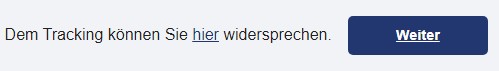
\includegraphics[width=\linewidth]{hochschule_cookie_banner}
\caption{Eigene Aufnahme des Tracking-Banners der Hochschule Mannheim~\autocite{HSMAWebsite2021}}
\label{fig:HSMATracking}
\end{figure}

\begin{figure}[!ht]
\centering
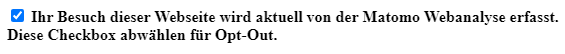
\includegraphics[width=\linewidth]{tracking_optout}
\caption{Eigene Aufnahme der Tracking Opt-Out Checkbox der Hochschule Mannheim~\autocite{HSMAWebsite2021}}
\label{fig:HSMAOptOut}
\end{figure}

Um \textit{Nudging} besser zu verstehen, betrachten wir ein Dark Pattern, welches sich auf der Homepage der Hochschule Mannheim finden lässt. In \autoref{fig:HSMATracking} ist ein Ausschnitt des Tracking-Banners der Hochschule Mannheim zu sehen. Die Zustimmung zu nicht essenziellem Tracking wird hinter einem prominent dargestelltem \textit{Weiter} Button verborgen. Um eine konträre Entscheidung zu treffen, muss der Nutzer auf den weit weniger prominenten \textit{hier} Link klicken. Dieser führt zu der Datenschutzerklärung der Hochschule in der nach der in \autoref{fig:HSMAOptOut} dargestellten Checkbox gesucht werden muss, um das Tracking zu deaktivieren. Auffällig ist, dass in dem Text das Wort \textit{tracking} nicht vorkommt. Hier wurden mehrere \textit{Nudges} genutzt, um den Nutzer dazu zu bewegen, das Tracking zu akzeptieren. Erst wird der Nutzer zum direkten Akzeptieren durch einen auffälligeren Button \textit{genudged}, danach wird der Nutzer durch das erschwerte Abwählen des Trackings in Richtung der Akzeptanz des Trackings \textit{genudged}.

Zusammenfassend lässt sich sagen, dass Dark Patterns als Zusammenschluss verschiedener Nudges verstanden werden kann.

\section{Kategorien von Dark Patterns}
//Bilder aus Kapitel 3. Nudging (HSMA) einordnen + zweites Dark Pattern (confirm shaming) direkt über \autoref{fig:HSMAOptOut}\\
// Taxonomy mit verschiedenen Quellen belegen \autocite*{Gray_2018,M.Bhoot2020,Brignull}
\subsection{Nagging}
// Nerven bis man ja sagt (Z.B. iPhone Apple Pay-Einrichtung or No Button for No)
\subsection{Behindernd}
// Roach motel, easy to enter hard to leave
\subsection{Irreführend}
\label{chap:Irreführend}
// Verbergen von Information durch Design, z.B. wenn ein Shop immer direkt die teuerste Variante (farblich) eines Produkts zeigt
\subsection{Heimlich}
// Versteckte Kosten, sneak into basket, versteckte Subscriptions, z.B. hinter einem free trial
\subsection{Zwingend}
// Wenn man gezwungen wird, etwas zu tun, was man nicht will und was nicht erforderlich ist, z.B. Annehmen eines Newsletters zur Anmeldung oder das Liken einer Seite, um sie zu besuchen


\section{Schutz vor Dark Patterns}
\subsection{Gesetzliche Einschränkungen}
// Self-regulate or get regulated
\subsection{Entwickler-Aufklärung}
// Entwickler entwickeln oft Dark Patterns ohne dass ihnen das bewusst ist
\subsection{Nutzer-Aufklärung}
// subreddit '/r/assholedesign' \autocite{Chivukula_2019}\\
// Brignull klärt auf seiner Seite auf \autocite{Brignull}
// Nutzer aufklären, führt zur Reduzierung des Erfolges von Dark Patterns, was wiederum dafür sorgt, dass Dark Patterns sich für Firmen weniger lohnen und sie auf diese verzichten\\
Laut \citeauthor{Brignull} \autocite{Brignull} ist der beste Schutz vor Dark Patterns, sie sich bewusst zu machen und die Firmen, die sie benutzen zu boykottieren. \autoref{chap:Psychologie} zeigt, dass der Mensch anfällig für Dark Patterns ist. \citeauthor{M.Bhoot2020} \autocite{M.Bhoot2020} fanden in einer Nutzerbefragung heraus, dass Nutzer Dark Patterns mit stark schwankender Konsistenz erkennen. Nur 18,6\% der Befragten haben das Roach Motel Dark Pattern erkannt. Deshalb ist es wichtig, Nutzer über die Dark Patterns aufzuklären, sodass sie diese leichter erkennen, um sich selbst vor ungewollten Konsequenzen zu schützen.

\section{Fazit und Ausblick}

\nocite{*}
% Literaturverzeichnis
\addcontentsline{toc}{section}{Literatur}
\printbibliography
\end{document}
// bill zitieren mit namen